\chapter{\evaluation}

Ebben a fejezetben kiértékelem munkámat mialatt megválaszolom a következő kérdéseket:

\begin{itemize}
	\item \textbf{Kérdés1}: Hogy aránylik egymáshoz az előfeldolgozás, a generálás és az utófeldolgozás időtartama?
	\item \textbf{Kérdés2}: Hogy skálázódik a generálás modell méret szempontjából?
	\item \textbf{Kérdés3}: Hogy skálázódik a generálás modell darabszám szempontjából?
	\item \textbf{Kérdés4}: Mennyire diverzek a lekérdezések? (egymás utáni 50 illetve 50 független) 
\end{itemize}

\section{Mérési környezet felállítása}


A méréseket eclipse fejlesztői környezetben végeztem. Ahhoz, hogy bemelegítsem a modell generátort memóriakezelés és optimalizálás szempontjából 5 extra futást adtam hozzá minden kiértékelt mérés előtt. A mérésekhez a generátor számára 4000 MB memóriát biztosítottam, és ez mindig elegendőnek bizonyult. Az összes mérést egy egyszerű asztali számítógépen végeztem (Intel Core i7-3520M CPU, 2.90GHz, Windows 10 Pro). A generáláshoz részmodellként egy 22 elemből álló ASG-t adtam meg, de csak az esszenciális részletek specifikálásával.  

\section{K1}
\subsection{Specifikáció}
A kérdés megválaszolásához 12 mérést végeztem, 50 példány gráfot generáltam 10 hozzáadott elemmel. A kölünböző futásidőket egy helyre összegyűjtöttem és az adatokat transzformáltam befogadható formátumra.
\subsection{Eredmények}
A mérés eredményei  \aref{fig:grafikon}. ábrán láthatóak. Az ábra segítségével azt szeretném bemutatni, hogy a különböző futásidők nagyságrendileg eltérnek egymástól. A grafikon vízszintes tengelyén pedig az ábrázolt négy érték össszegét tekintjük 100 százaléknak.

A négy ábrázolt érték pedig rendre: Az utófeldogozás ideje(kék), a fordítás idejének század része (narancs), a generálás idejének tízezrede (szürke), és az előfeldolgozás idejének százmilliomoda (sárga). Tehát ezek szerint a különböző tényezők aránya a következő:
\begin{itemize}
	\item utófeldolgozási idő * 10 ~ fordítási idő * 2
	\item fordítási idő * 3 * 1000 ~ generációs idő
	\item generációs idő *  1000 ~ előfeldolgozási idő
\end{itemize}

\begin{figure}
	\centering
	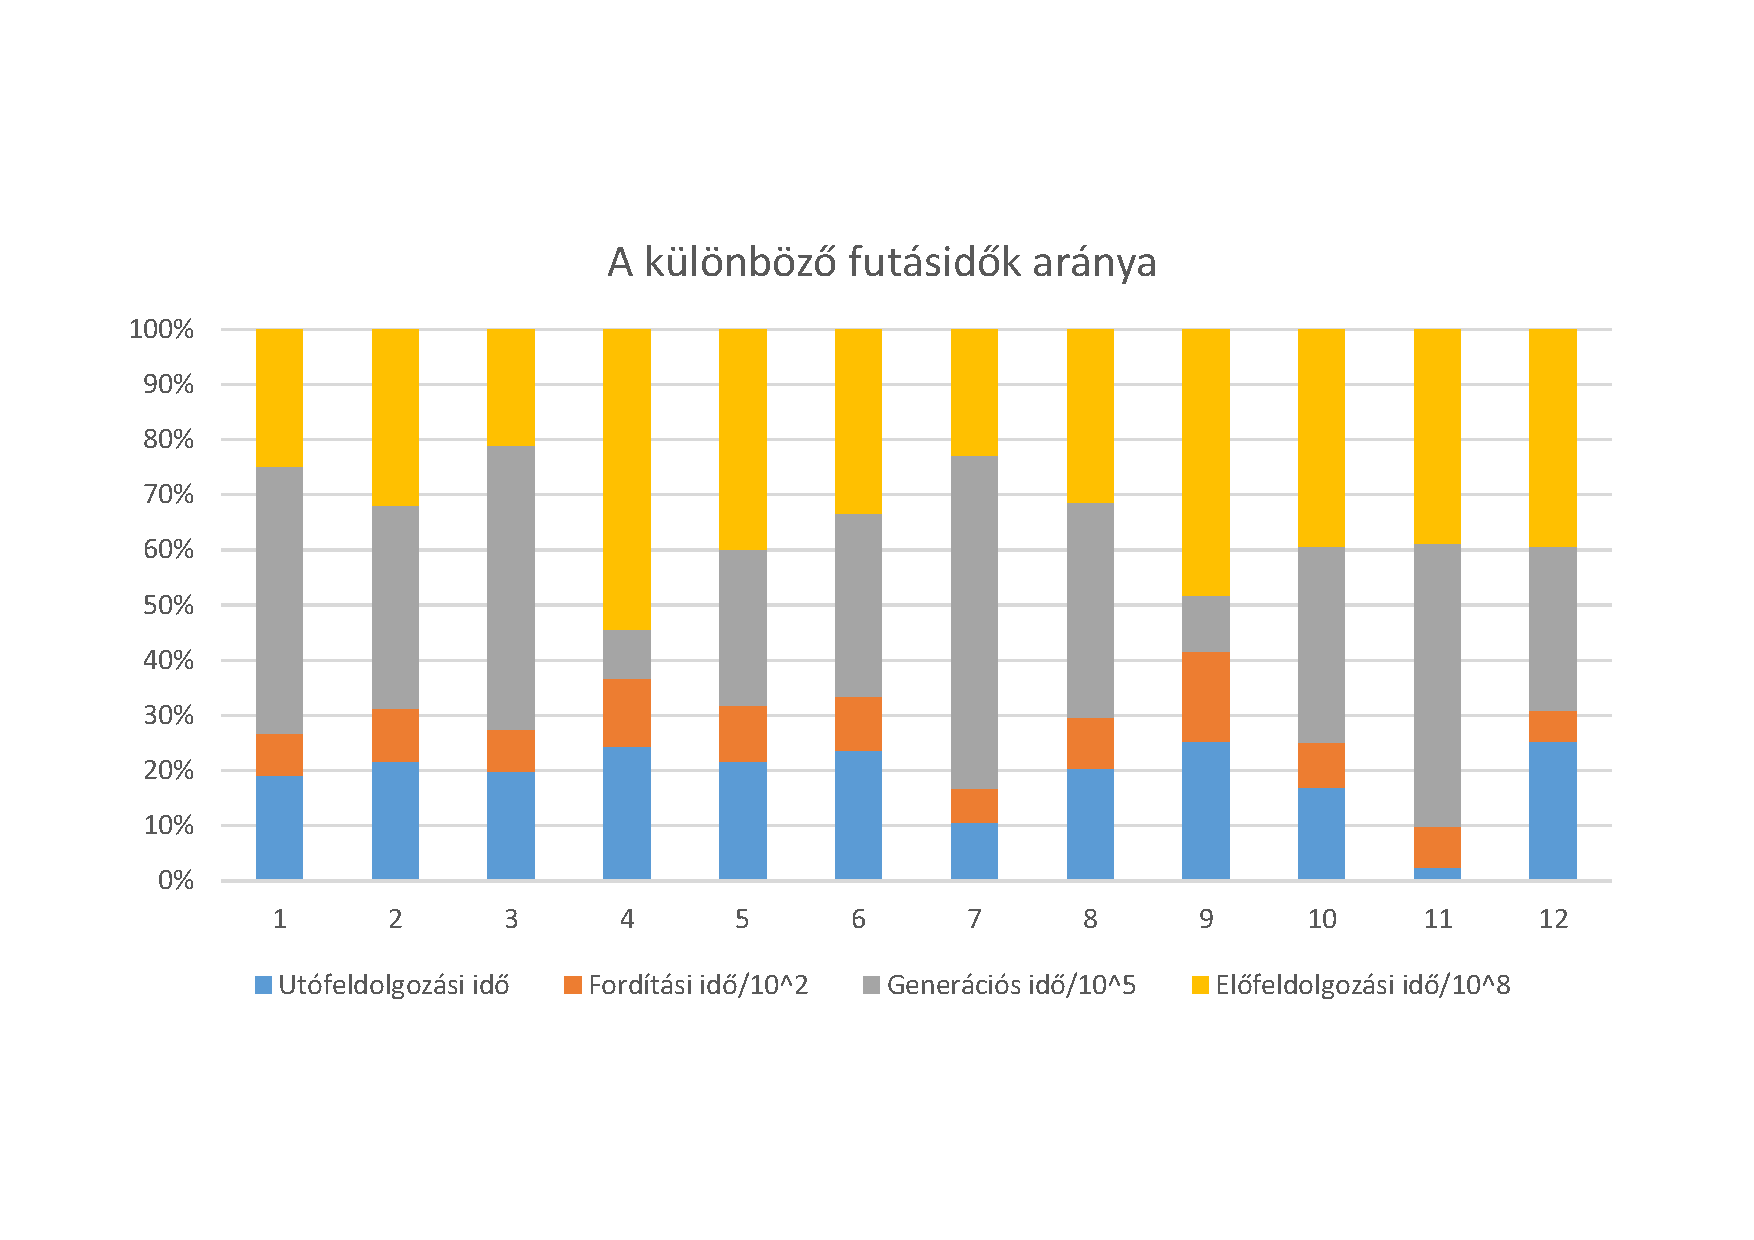
\includegraphics[width=1\textwidth]{figures/aránygrafikontáblázathelyett}
	\caption{A K1 mérés eredményei}
	\label{fig:grafikon}
\end{figure}



\section{K2}
\subsection{Specifikáció}
A kérdés megválaszolásához 3 al mérést végeztem. A három mérés egymástól csak a generált modellek minimális méretében különbözött, az elsőben 10 a másodikban 20 a harmadikban pedig 30 elemet generáltam a részmodellben megadottak mellé. 
Mindhárom almérést 12 alkalommal végeztem el, és minden alkalommal 50 példányt generáltam. 

\subsection{Eredmények}
A mérés eredményei \aref{fig:AmeresEredmeny}. ábrán láthatóak.


\begin{figure}
	\centering
	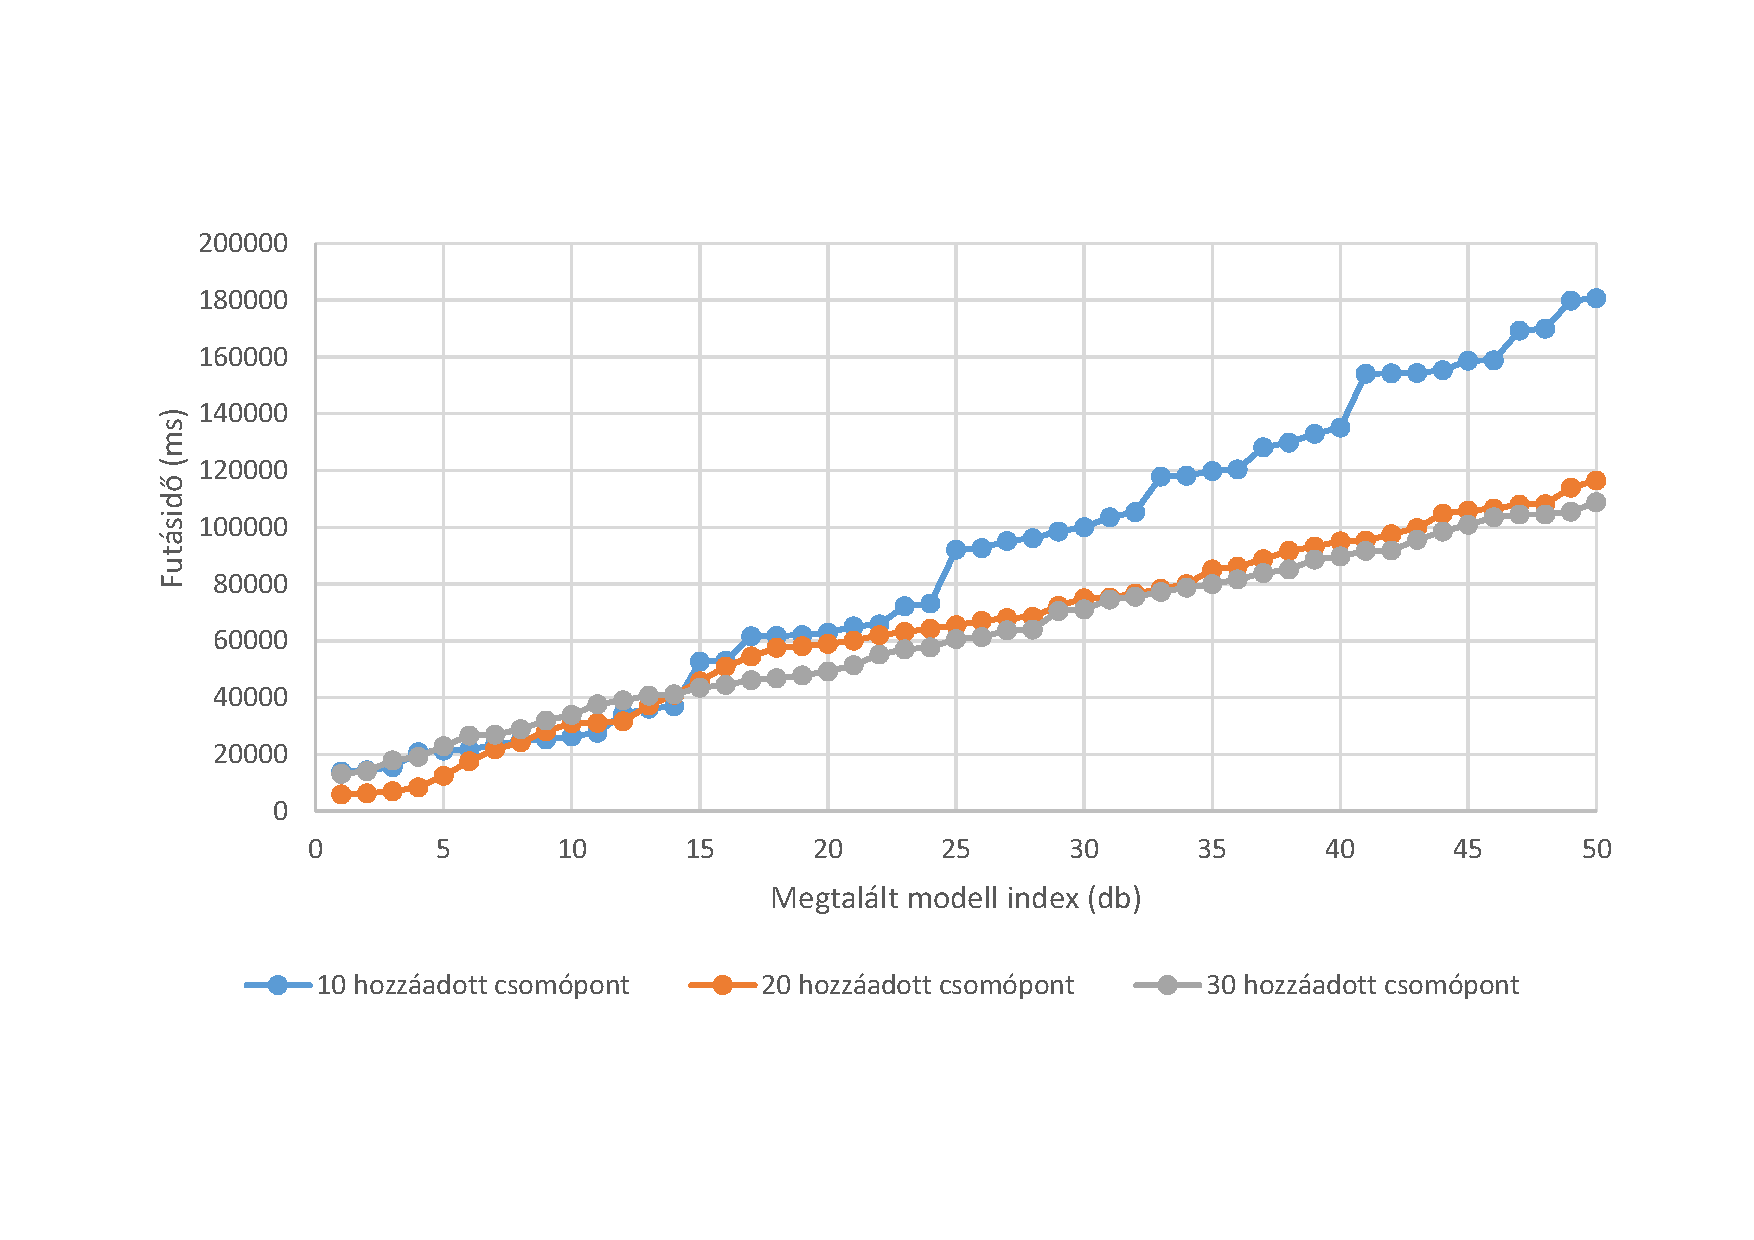
\includegraphics[width=1\textwidth]{figures/AmeresEredmeny}
	\caption{A K2 mérés eredményei}
	\label{fig:AmeresEredmeny}
\end{figure}

Az 50 darab generált modell megtalálásának ideje nem volt azonos a 12 alkalommal, ezértt a 12 érték mediánját kiválasztottam, az ábrán ezen medián értékek táthatóak. A 3 almérés eredményeit 3 színnel jelöltem. Az ábrán a vízszintes tengelyen a modellek láthatóak a megtalálás sorrendjében, a függőleges tengelyen pedig a futásidők mediánja milliszekundumban. 

A  három mérés eredményei külön-külön megfeleltethetőek egy egyenes trendvonalnak. Az egyre későbbi modellek megtalálása a diverzitás biztosítása miatt növekszik, egyre nehezebb ugyanis szignifikánsan különböző modelleket találni.

Az ábrán látható, hogy a generátor nehezebben boldogult a kis modellek megtalálásával  mint a nagyokéval. Ez azzal magyarázható, hogy a megadott részmodell elég nagy,(22 elem) emiatt tovább kell keresgélni, hogy 10 hozzáadott elemből ki tudja tölteni az összes szükséges  helyet és még különböző is legyen. 


K3 : B(12x, 1db, 5-10-15-...50), B+(12x, 10, 5-10-15-...50) , B++=(12x, 30, 5-10-15-...50) 
\section{K3}
\subsection{Specifikáció} 
A kérdés megválaszolásához 13 al mérést végeztem. Minden al mérést 10 alkalommal végeztem el, és minden alkalommal 10 példány modellt generáltam. A 13 mérés során rendre 5, 10 ,15, ...,50, 100, 150, 200 elemet adtam hozzá a részmodellhez.

\subsection{Eredmények}
A mérés eredményei \aref{fig:BmeresEredmeny}. ábrán láthatóak.   

\begin{figure}
	\centering
	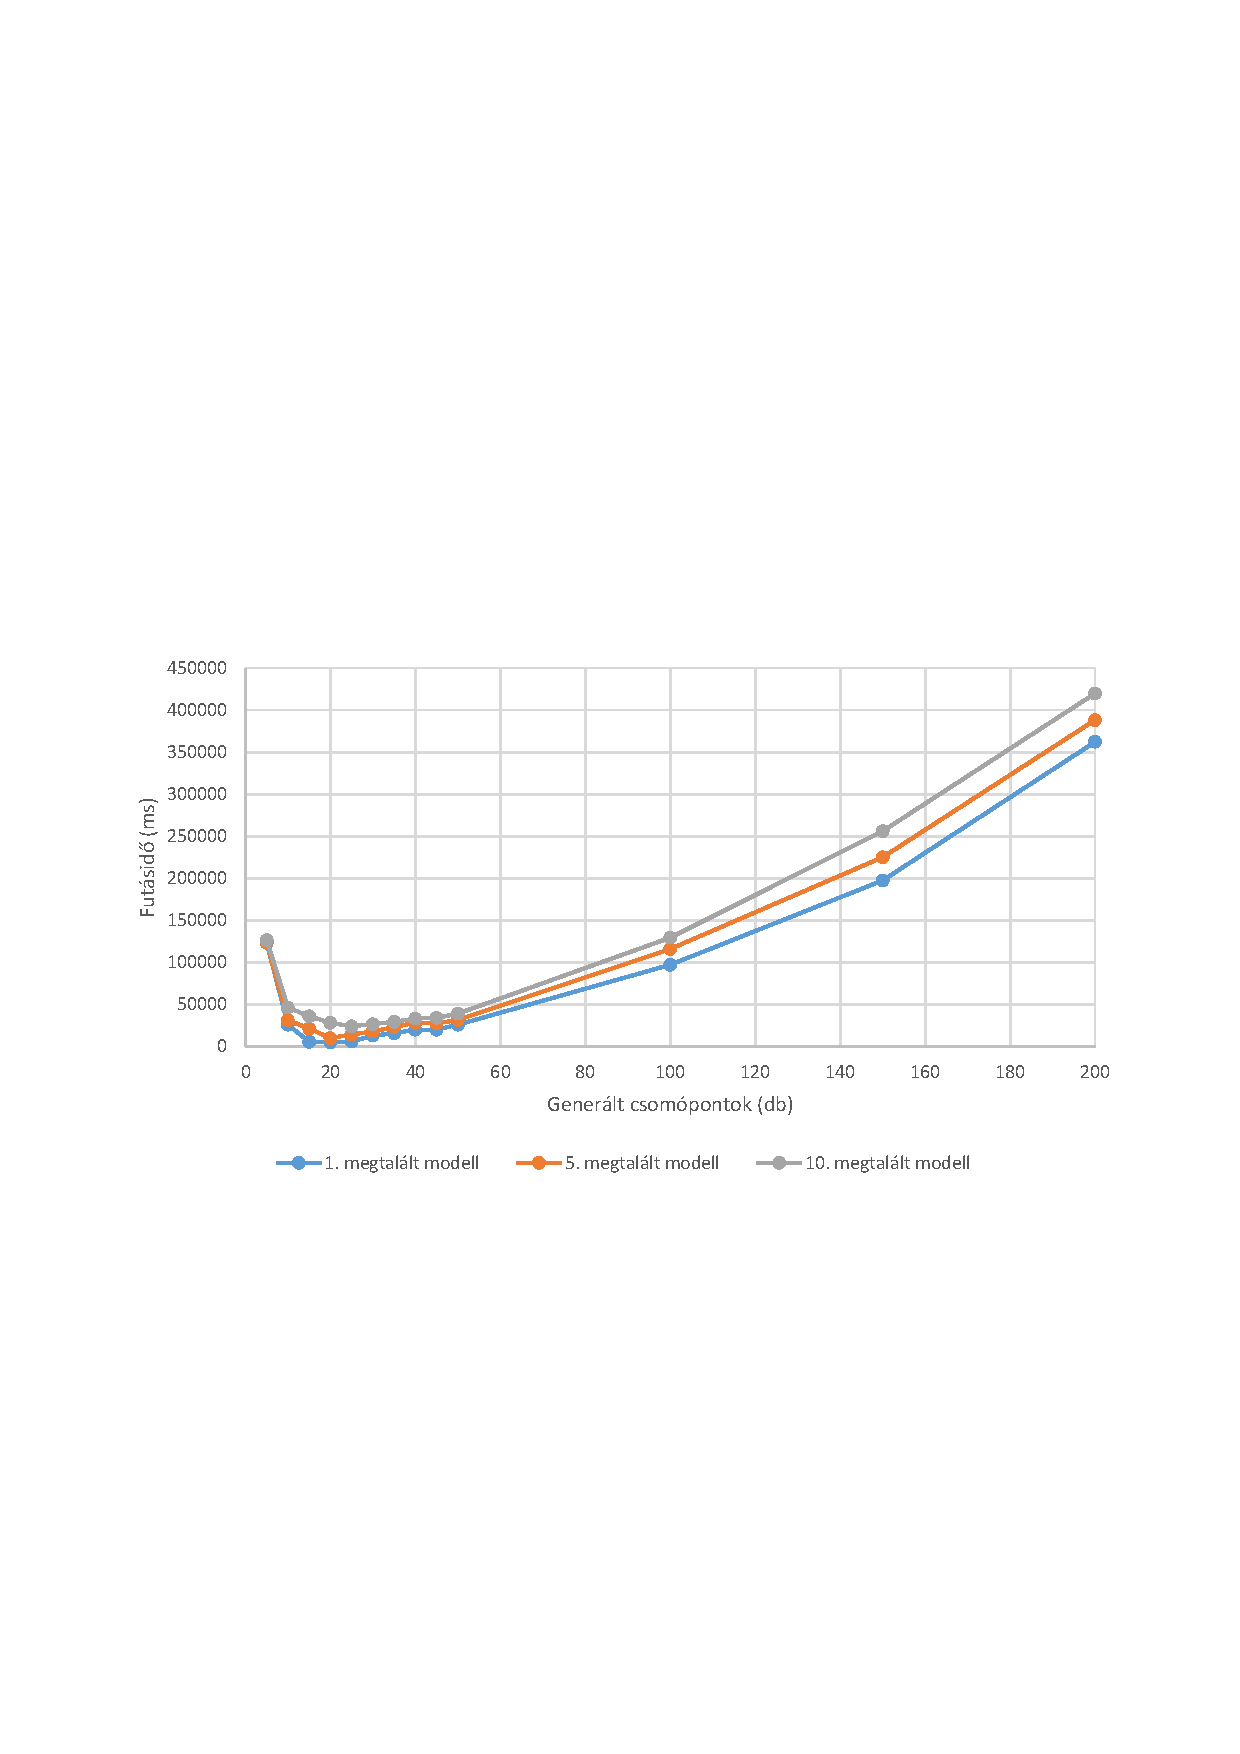
\includegraphics[width=1\textwidth]{figures/statisticsPlottal1}
	\caption{A K3 mérés eredményei}
	\label{fig:BmeresEredmeny}
\end{figure}

Mind a 13 alkalommal vizsgáltam az 1., az 5. és a 10. modell megtalálásához szükséges időt. Az előző méréshez hasonlóan most is rendre a 12 identikus mérés futásidejének mediánját ábrázoltam. A vízszintes tengelyen a hozzáadott elemek darabszáma, míg a függőleges tengelyen az adott modell megtalálásához szükséges futásidő látható. 

Itt is látható, hogy a kis darabszámú generált elem hozzáadásával nehezebben boldogult a generátor, mint a közepes elemszámokkal, ám a hatalmas modellek megtalálása is egyre nehezebb feladatnak bizonyult. Ha a 3 görbéhez illeszkedő trendvonalat keresünk és az elejét vagy a végét levágjuk, akkor egy köbös függvényt tudunk illeszteni a szakaszokra. 
Mit a legtöbb np teljes problémára erre is igaz, hogy a megfelelő egyszerűsítésekkel és megoldásokkal exponenciális helyet köbösre egyszerűsítődik le a probléma.  

A három vonal ezen kívül azt is mutatja, hogy az első modellt gyorsabb megtalálni mint az 5-et, és az 5.-et gyorsabb mint a 10.-et. Ez továbbra is a diverzitás fenntartásának nehézségéből fakad.


\section{Diverzitás mérése}